\chapter{Постановка задачи и обзор решений} \label{ch1}
\textit{Задача фокусировки} -- нахождение положения линзы или системы линз, в котором снимок объекта будет максимально четким, то есть наведение объекта схемки на резкость.

\textit{Автофокусировка} -- фокусировка, которая осуществляется алгоритмом без участия человека.

\textit{Цифровой микроскоп} -- вид оптического (светового) микроскопа, в котором для наблюдения объекта используется цифровая камера вместо окуляров или вместе с ними.

Необходимо исследовать существующие решения, выявить их достоинства и недостатки, а также разработать алгоритм автофокусировки цифрового микроскопа, который отличался бы простотой внедрения, высокими скоростью работы и метриками качества даже при наличии шума. Кроме того, алгоритм должен работать исключительно с изображениями с камеры, то есть без применения каких-либо дополнительных датчиков.

\section{Существующие классические методы автофокусировки} \label{ch1:sec1}
Существует множество классических методов автофокусировки. Например, контрастный, фазовый (Phase-Detection Autofocus или PDAF) или аналитический метод на основе оценки резкости изображения. В этом параграфе будут рассмотрены их алгоритмы работы.

\subsection{Контрастный автофокус}
Контрастный автофокус является наиболее простым и примитивным, но из-за этого наименее эффективным. Работает он следующим образом: камера перемещается в несколько различных положений и в каждом из них вычисляется контрастность. Эту величину можно рассчитать несколькими способами. Пусть размер изображения равен $N \times M$, тогда пиксели имеют номера $(i,j),\ 1 \leq i \leq N,\ 1 \leq j \leq M$. Контрастность можно вычислить по одной из следующих формул:

\begin{enumerate}[1.]
	\item \begin{equation}
		\gamma = \dfrac{B_{max} - B_{min}}{B_{max} + B_{min}},
	\end{equation}
	где $B_{max} = \max\limits_{i,j} B_{ij},\ B_{min} = \min\limits_{i,j} B_{ij}$ -- максимальная и минимальная яркость изображения соответственно.
	
	\item \begin{equation}
		\gamma = \sqrt{\dfrac{1}{NM} \sum\limits_{i=1}^{N} \sum\limits_{j=1}^{M} (B_{ij} - \overline{B})^2},
	\end{equation}
	где $\overline{B} = \dfrac{1}{NM} \sum\limits_{i=1}^{N} \sum\limits_{j=1}^{M} B_{ij}$ -- средняя яркость изображения.
\end{enumerate}

Далее выбирается то положение камеры, в котором контрастность максимальна. В случае идеального изображения зависимость контрастности от положения линзы должна быть симметричной и гладкой, напоминающей нормальное распределение. Однако наличие шумов может приводить к локальным максимумам. Чтобы избежать попадания в локальный максимум, производится достаточно много дополнительных перемещений. 

Алгоритм контрастного автофокуса обладает несколькими существенными минусами:
\begin{itemize}
	\item Нельзя определить верное направление движения камеры
	\item Приходится делать много промежуточных перемещений
	\item Алгоритм чувствителен к шуму
	\item Текстура объекта может сильно влиять на результат
\end{itemize}

Среди достоинств данного метода легкая реализация, неплохая точность, учитывая простоту вычислений.

\subsection{Метод анализа резкости}
Метод, о котором пойдет речь в этом параграфе, работает схожим с контрастным автофокусом образом, но вычисляет другую величину. Данный алгоритм работает на основе расчета резкости изображения. Сама же резкость рассчитывается путем нахождения дисперсии лапласиана в каждой точке снимка. 

Лапласиан является мерой второй производной и используется для поиска областей с быстрой сменой интенсивности. Чем выше дисперсия Лапласиана по всему изображению, тем выше <<четкость>> этого изображения. Аналитически лапласиан определяется формулой
\begin{equation}
	L=\frac{\partial^2 f}{\partial x^2} + \frac{\partial^2 f}{\partial y^2}
\end{equation}

Однако при работе с изображением, то есть с многомерными массивами чисел, возникает трудность в применении данной формулы, так как нет явной функции, которая описывала бы сделанный снимок. Чтобы решить эту проблему, необходимо более детально рассмотреть, что из себя представляет лапласиан. Лапласиан есть дивергенция градиента заданной функции:
\begin{equation}
	L = \nabla F = \text{div}\ \text{grad} F
\end{equation}

Приблизительно рассчитать градиент в точке можно с помощью оператора Собеля \cite{SobelOperator}. Оператор Собеля представляет собой дискретный дифференциальный оператор, вычисляющий приближённое значение градиента яркости изображения. Данный оператор производит свертку исходного изображения с ядрами размера $3 \times 3$.

Пусть \textbf{A} -- исходное изображение, $\textbf{G}_x$ и $\textbf{G}_y$ -- изображения, каждая точка которых является приблизительным значением производной по $x$ и $y$ соответственно.
\begin{equation}
	\textbf{G}_x =
	\begin{bmatrix}
		-1 & 0 & +1\\
		-2 & 0 & +2\\
		-1 & 0 & +1
	\end{bmatrix}
	\circledast \textbf{A},\ 
	\textbf{G}_y =
	\begin{bmatrix}
		+1 & +2 & +1\\
		0 & 0 & 0\\
		-1 & -2 & -1
	\end{bmatrix}
	\circledast \textbf{A},
\end{equation}
где $\circledast$ -- операция свертки.

\begin{equation}
	\textbf{G} = \sqrt{\textbf{G}_x^2 + \textbf{G}_y^2}
\end{equation}

Матрица \textbf{G} описывает значение градиента в каждом пикселе. Однако для дальнейшего шага потребуются матрицы $\textbf{G}_x, \textbf{G}_y$. Далее нужно посчитать дивергенцию полученного градиента. Для каждой матрицы градиента необходимо посчитать приблизительное значение дивергенции по каждой координате. Для каждого пикселя в матрице вычислим его частную производную. Это можно сделать, вычислив разницу между значением этого пикселя и средним значением его соседей без учета диагональных.

\begin{equation}
	\text{div} f_{i,j} = f_{i,j} - \dfrac{f_{i-1,j} + f_{i+1,j} + f_{i,j-1} + f_{i,j+1}}{4}
\end{equation}

Получив две матрицы дивергенции, необходимо их сложить, чтобы получить матрицу лапласиана. 
\begin{equation}
	L = \nabla F = \text{div} \textbf{G} = \frac{\partial \textbf{G}_x}{\partial x} + \frac{\partial \textbf{G}_y}{\partial y}
\end{equation}

Следующим этапом после вычисления матрицы лапласиана является нахождение выборочной дисперсии значений этой матрицы. Именно это значение и будет мерой четкости/резкости изображения.

Для того, чтобы определить положение фокуса, необходимо проделать упомянутые выше шаги для набора снимков, сделанных в разных фокальных плоскостях, и выбрать тот, который имеет наибольшее по абсолютной величине значение дисперсии лапласиана, так как это будет означать максимальные перепады интенсивности, а значит, наиболее выраженные края и границы объекта съемки.

Очевидно, этот подход имеет несколько недостатков:
\begin{itemize}
	\item Малая скорость работы. Алгоритм требует целого набора изображений на вход, что приводит ко множественным перемещениям камеры.
	\item Как и в случае контрастного автофокуса, для большого увеличения потребуется большее число замеров и снимков. Иногда параметры для каждого объектива определяются вручную, но так или иначе метод зависим от оптики.
	\item Точность этого метода остается невысокой. После работы алгоритма часто требуется ручная корректировка.
%	\item Индивидуальная настройка для каждого объектива/камеры. Необходимо сделать серию снимков, выбрать самый качественный из них и вернуть камеру в это положение. Очевидно, что для объективов с большим коэффициентом увеличения разница положений камеры между двумя соседними снимками должна быть меньше, чем для объективов с малым увеличением. При этом диапазон расстояний для любой конфигурации должен быть примерно одинаковым.
%	\item Невысокая точность. У данного алгоритма она ограничивается шагом сдвига камеры по оси $z$, так как истинное положение фокальной плоскости может оказаться между двумя зарегистрированными положениями камеры. Тогда в худшем случае ошибка вычисления составит $\dfrac{s}{2}$, где $s$ -- величина шага по вертикали.
\end{itemize}

Стоит отметить, что автофокус на основе анализа резкости более устойчив к неравномерной структуре объекта съемки, разному освещению и наличию шумов, чем контрастный автофокус.

\subsection{Фазовый автофокус} % ~ нужен, чтобы избавиться от висячего предлога (союза) в конце строки
\begin{figure}[ht!] 
	\center
	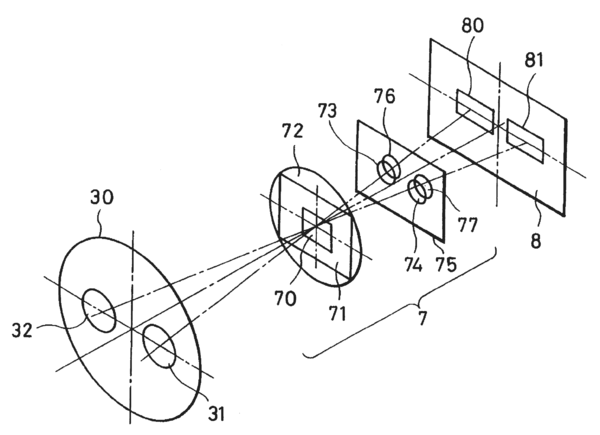
\includegraphics [scale=1] {my_folder/images/phase_focus_detecror.png}
	\caption{Устройство фазового автофокуса. 72 - конденсор; 8 - датчик; 80, 81 - ПЗС-линейки; 30 - зрачок объектива; 31, 32 - области зрачка; 75 - маска; 76, 77 - микрообъективы для датчика; 70 - окно, ограничивающее размер изображения; 71 - рамка конденсора.}
	\label{fig:pdaf}
\end{figure}

Принцип работы фазового автофокуса следующий: в матрицу (\firef{fig:pdaf}) встроен фазовый датчик (8) с двумя линейками (80, 81), в которые приходят световые потоки с противоположных областей (31 и 32) зрачка (30) объектива через микрообъективы (76 и 77). Если объект в фокусе,  изображения объекта находятся в центрах соседних ПЗС-линеек \cite{носов1986основы}. Таким образом, сигналы, получаемые процессором с разных линеек, совпадают (находятся <<в фазе>>). Если же объектив не сфокусирован на объекте съемки, то изображения смещаются внутрь или наружу линеек. Сигналы перестают совпадать и имеют разность фаз (\firef{fig:phase_images}). На основе этой разности фаз считается фазовый сдвиг, а далее -- необходимое смещение для системы линз.

\begin{figure}[!htbp]
	\begin{subfigure}[t]{0.45\linewidth}
		\centering
		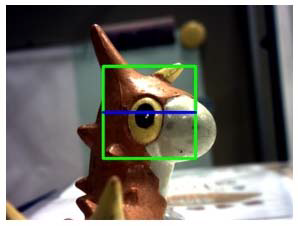
\includegraphics[width=.85\linewidth]{my_folder/images/phase_image_1}
		\caption{}
		\label{fig:phase_image-a}
	\end{subfigure}
	\hfill
	\begin{subfigure}[t]{0.45\linewidth}
		\centering
		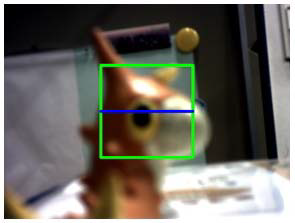
\includegraphics[width=.85\linewidth]{my_folder/images/phase_image_2}
		\caption{}
		\label{fig:phase_image-b}
	\end{subfigure}
	\\
	\begin{subfigure}[t]{0.45\linewidth}
		\centering
		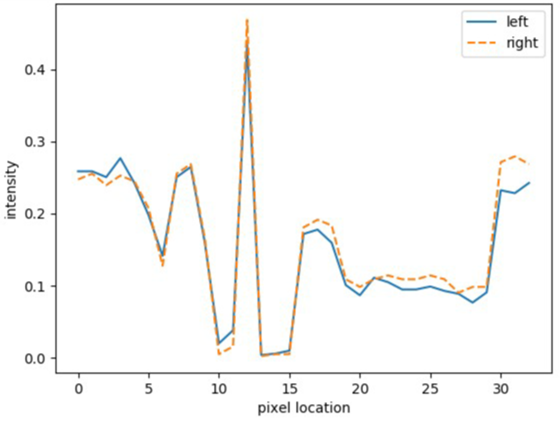
\includegraphics[width=.85\linewidth]{my_folder/images/phase_image_3}
		\caption{}
		\label{fig:phase_image-c}
	\end{subfigure}
	\hfill
	\begin{subfigure}[t]{0.45\linewidth}
		\centering
		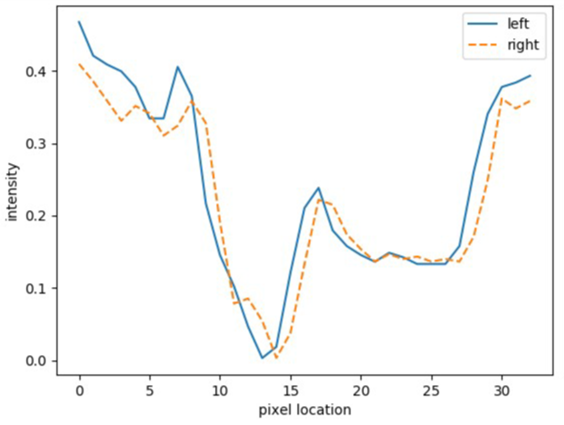
\includegraphics[width=.85\linewidth]{my_folder/images/phase_image_4}
		\caption{}
		\label{fig:phase_image-d}
	\end{subfigure}
	\caption{Снимки и срезы их фазовых изображений: {\itshape a} --- снимок объекта в фокусе; {\itshape b} --- снимок объекта не в фокусе; {\itshape c} --- срез фазового изображения, когда объект в фокусе; {\itshape d} --- срез фазового изображения, когда объект не в фокусе}
	\label{fig:phase_images}  
\end{figure}

Фазовый сдвиг положителен, если фокальная плоскость находится перед объектом, и отрицателен, если фокальная плоскость находится позади объекта. Чем дальше объект от фокальной плоскости, тем больше абсолютная величина фазового сдвига.

Однако оценка фазового сдвига редко бывает безошибочной. Шум датчика, размытие изображения часто влияют на точность оценки фазового сдвига. Хотя ошибку этой оценки можно уменьшить, применив фильтр Гаусса к фазовой корреляции, по-прежнему трудно получить точную оценку фазового сдвига, когда объектив находится далеко от сфокусированного положения линзы. Другая серьезная проблема PDAF заключается в том, что ошибка оценки фазового сдвига может накапливаться в процессе принятия решения о движении линзы.

Для оценки фазового сдвига обычно используется фазовая корреляция. Она применяется для поиска соответствия между смещенными, повернутыми и разномасштабными изображениями. Но этот метод может легко потерпеть неудачу при работе с размытыми или зашумленными изображениями.

В параксиальном и тонколинзовом приближениях формирования изображения глубина объекта D связана с фазовым сдвигом s соотношением \cite{AF-Net}
\begin{equation}
	s = A\left( \frac{1}{z} - \frac{1}{D}\right),
	\label{eq:p_phase_shift_s}
\end{equation}
где $A$ -- некоторая константа, $z$ -- расстояние от фокальной плоскости до линзы. Когда объект находится в фокусе, $z = D$. Однако уравнение (\ref{eq:p_phase_shift_s}) может часто не выполняться при наличии ошибки оценки фазового сдвига. К этому могут приводить ситуация, когда левый и правый фазовые датчики расположены слишком далеко друг от друга, а также наличие шума и искажений от оптики.

В качестве решения данной проблемы предлагается использовать статистический метод, который сначала получает распределение вероятностей оптимального расстояния хода линзы для заданного фазового сдвига на этапе калибровки, а затем использует его для определения расстояния хода линзы при тестировании. Это поможет ускорить процесс автофокусировки, однако такая калибровка потребуется для каждого объектива.

\subsection{Фазовый сдвиг}
Для идеальной пары левого и правого фазового изображения с фазовым сдвигом $\Delta x$ выполняется следующее:
\begin{equation}
	r(x, y) = l(x + \Delta x, y),
\end{equation}
где $(x, y)$ -- координаты пикселя, $r(\cdot,\cdot)$ и $l(\cdot,\cdot)$ -- правое и левое фазовые изображения соответственно.

Фазовый сдвиг между левым и правым изображениями можно получить с помощью фазовой корреляции \cite{PhaseCorrelation}. Пусть $L$ и $R$ -- двумерное преобразование Фурье для левого и правого фазовых изображений соответственно. На первом шаге найдем корреляционную матрицу $p(x, y)$.
\begin{equation}
	p(x, y) = F^{-1} \left\{ \frac{L \circ \overline{R}}{\left| L \circ R \right|} \right\}
\end{equation}
где $F^{-1}$ -- обратное двумерное преобразование Фурье, <<$\circ$>> -- поэлементное умножение матриц, <<$\overline{\cdot}$>> -- комплексное сопряжение.

Далее рассматриваем корреляционную прямую $p(x,0)$. Аргумент $y$ принят равным нулю, поскольку в матрице значение $p(x,y)$ соответствует корреляции при сдвиге на $x$ и $y$ по соответствующим осям. В данном случае сдвиг производится лишь по одной оси, поэтому второй аргумент равен нулю. Однако шум от датчиков может приводить к нескольким пикам в корреляционной матрице. Чтобы этого избежать, применим сглаживание корреляционной кривой $p(x,0)$ Гауссовым ядром $g(x)$:
\begin{equation}
	p_f(x) = g(x) * p(x, 0),
\end{equation}
где $p_f(x)$ -- исправленная корреляционная кривая. Тогда фазовый сдвиг $\Delta x$ определяется как
\begin{equation}
	\Delta x = \text{arg} \max_x p_f(x)
\end{equation} 

Если построить график фазового сдвига в зависимости от положения линзы, полученная кривая будет называться профилем фазового сдвига. Положение линзы, соответствующее нулевому фазовому сдвигу, является положением линзы в фокусе. Аналогично, если мы построим график контрастности изображения в зависимости от положения линзы, получим профиль фокуса (\firef{fig:phse_profile}). На нем положение линзы в фокусе соответствует максимальному значению контрастности и оно примерно совпадает с нулевым фазовым сдвигом.

\begin{figure}[ht!] 
	\center
	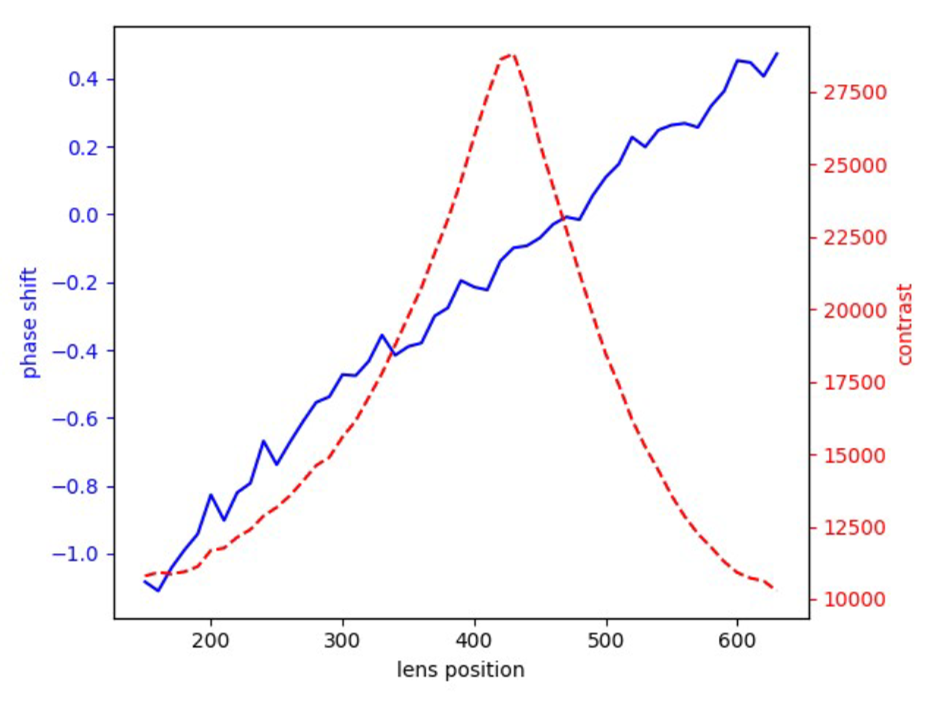
\includegraphics [scale=0.7] {my_folder/images/phase_profile.png}
	\caption{Фазовый профиль и профиль фокуса}
	\label{fig:phse_profile}
\end{figure}

\section{Нейросетевые методы} \label{ch1:sec2} 
Фазовый автофокус показывал отличные результаты по сравнению с более старыми методами автофокусировки. Но упомянутые выше недостатки, в частности неустойчивость к шуму, побуждали искать новые методы работы с оптикой и камерами. Кроме того с ростом интереса к нейросетям и машинному обучению были предприняты попытки использовать их и в этой области. Было предложено несколько решений, использующих глубокое обучение. Некоторые из них определяли смещение камеры на основе разности двух изображений \cite{RaiDastidar}, другие по двум снимкам генерировали новое четкое изображение \cite{li2020rapid}. Однако для уменьшения временных затрат на фокусировку исследования также были направлены на разработку методов, которые требуют только одного снимка с камеры для начала работы, и минимального общего количества перемещений. Так была разработана сверточная нейронная сеть на основе алгоритма фазового автофокуса AF-Net.

\subsection{Нейросеть AF-Net}
Подход на основе глубокого обучения \cite{AF-Net} позволяет уменьшить влияние шума и ошибку, которая может накапливаться при выполнении большого числа операций с фазовыми изображениями.

На вход нейросети посутпают те же фазовые изображения (левое и правое), на выходе получается вещественное число со знаком, которое обозначает направление и величину смещения линзы для достижения состояния максимальной четкости. Архитектура сети показана в \taref{tab:AFNet_struct}:

\begin{table}[!htbp]
	\centering
	\small
	\begin{tabular}{|p{2.5cm}<{\centering}|p{2.5cm}<{\centering}|p{2.5cm}<{\centering}|p{3.5cm}<{\centering}|p{3.5cm}<{\centering}|}
		\hline
		\multicolumn{5}{|c|}{Выделение признаков} \\ \hline
		Названия слоя & Ядро & Шаг ядра & входные/выходные каналы & входной/выходной размер\\ \hline
		conv0 & $5 \times 5$ & $2 \times 2$ & 2/64 & $33 \times 33$/ $16 \times 16$ \\ \hline
		conv1 & $3 \times 3$ & $1 \times 1$ & 64/128 & $16 \times 16$/ $16 \times 16$ \\ \hline
		conv2 & $3 \times 3$ & $2 \times 2$ & 128/128 & $16 \times 16$/ $8 \times 8$ \\ \hline
		conv2 & $3 \times 3$ & $2 \times 2$ & 128/256 & $8 \times 8$/ $4 \times 4$ \\ \hline
		\multicolumn{5}{|c|}{Полносвязные слои} \\ \hline
		Название слоя & \multicolumn{2}{c|}{Входные/выходные размеры} & \multicolumn{2}{c|}{Функция активации} \\ \hline
		fc0 & \multicolumn{2}{c|}{4096/256} & \multicolumn{2}{c|}{ReLU} \\ \hline
		fc1 & \multicolumn{2}{c|}{256/64} & \multicolumn{2}{c|}{ReLU} \\ \hline
		fc2 & \multicolumn{2}{c|}{64/1} & \multicolumn{2}{c|}{Линейная} \\ \hline
	\end{tabular}
	\caption{Архитектура нейросети}
	\label{tab:AFNet_struct}
\end{table}

После каждого сверточного слоя следует функция активации ReLU и пакетная нормализация (batch normalization). Используется оптимизатор Adamax, размер батча равен 128, параметры оптимизатора $\beta_1 = 0.5,\ \beta_2 = 0.999$, Скорость обучения (или learning rate) равна 0.001. Использовалась ранняя остановка, если значение функции потерь не уменьшалось существенно в течение 20 эпох. В среднем процесс обучения задействует 80 эпох.

\section{Сравнение статистического и нейросетевого метода}
Сравним AF-Net с классическим методом фазового автофокуса, используя следующие метрики: коэффициент успеха (success rate), количество перемещений линзы до остановки процесса и ошибка конечного положения линзы. Сравним на разных начальных положениях линзы. Обозначим нулем положение линзы в фокусе, положительное смещение - это перемещение линзы ближе к объекту, отрицательное - дальше от объекта, чем положение в фокусе. Результаты сравнения по указанным метрикам приведены в \taref{tab:Comparison}. Так как важным показателем является скорость работы метода, то рассмотрим сравнение их производительности в \taref{tab:performance}

\begin{table}[!htbp]
	\centering
	\small
	\begin{tabular}{|c|c|c|c|c|c|c|c|}
		\hline
		\multirow{2}{*}{Метод}& \multirow{2}{*}{Метрика} & \multicolumn{6}{c|}{начальное положение линзы} \\
		\cline{3-8} & & -30 & -20 & -10 & 10 & 20 & 30\\ \hline
		\multirow{3}{*}{AF-Net} & Success rate & 90.48 & 94.83 & 95.06 & 97.26 & 100.0 & 100.0\\ 
		\cline{2-8} & final lens position error & 1.381 & 1.207 & 1.185 & 1.027 & 0.981 & 0.826 \\
		\cline{2-8} & number of lens movements & 2.26 & 2.20 & 2.03 & 2.06 & 2.06 & 2.00\\ \hline
		\multirow{3}{*}{Статистический} & Success rate & 23.81 & 46.55 & 51.85 & 63.01 & 57.41 & 43.48\\ 
		\cline{2-8} & final lens position error & 10.57 & 5.741 & 4.000 & 3.342 & 3.426 & 3.261 \\
		\cline{2-8} & number of lens movements & 3.40 & 3.00 & 2.21 & 2.21 & 2.54 & 2.60\\ \hline
	\end{tabular}
	\caption{Сравнение метрик AF-Net и статистического метода}
	\label{tab:Comparison}
\end{table}

Также сравним их производительность:

\begin{table}[!htbp]
	\centering
	\small
	\begin{tabular}{|c|p{4cm}<{\centering}|p{4cm}<{\centering}|p{4cm}<{\centering}|}
		\hline
		Метод & Максимальная ошибка положения линзы & Максимальное количество перемещений линзы & Среднее время расчета одного перемещения (мс)\\ \hline
		AF-Net & 5 & 4 & 10.8\\ \hline
		Статистический & 12 & 7 & 28.3 \\ \hline
	\end{tabular}
	\caption{Оценка производительности}
	\label{tab:performance}
\end{table}


\section{Выводы} \label{ch1:conclusion}

Из сводных сравнительных таблиц хорошо видно, что нейросетевой подход превосходит классический как в метриках качества, так и по производительности. Это означает, что применение AF-Net оправдано, и благодаря ему, фокусировка будет проходить быстрее и точнее. Но автофокусировка, основанная на фазовых изображениях и фазовом сдвиге, имеет существенный недостаток -- она требует интеграции непосредственно в камеру, так как предполагается, что такой алгоритм является частью ПО камеры. Он использует показания фазовых датчиков. Но зачастую подключиться к ним извне нет возможности, или же эти датчики отсутствуют вовсе.